\documentclass{sigchi}

% Use this command to override the default ACM copyright statement (e.g. for preprints). 
% Consult the conference website for the camera-ready copyright statement.


%% EXAMPLE BEGIN -- HOW TO OVERRIDE THE DEFAULT COPYRIGHT STRIP -- (July 22, 2013 - Paul Baumann)
% \toappear{Permission to make digital or hard copies of all or part of this work for personal or classroom use is 	granted without fee provided that copies are not made or distributed for profit or commercial advantage and that copies bear this notice and the full citation on the first page. Copyrights for components of this work owned by others than ACM must be honored. Abstracting with credit is permitted. To copy otherwise, or republish, to post on servers or to redistribute to lists, requires prior specific permission and/or a fee. Request permissions from permissions@acm.org. \\
% {\emph{CHI'14}}, April 26--May 1, 2014, Toronto, Canada. \\
% Copyright \copyright~2014 ACM ISBN/14/04...\$15.00. \\
% DOI string from ACM form confirmation}
%% EXAMPLE END -- HOW TO OVERRIDE THE DEFAULT COPYRIGHT STRIP -- (July 22, 2013 - Paul Baumann)


% Arabic page numbers for submission. 
% Remove this line to eliminate page numbers for the camera ready copy
\pagenumbering{arabic}


% Load basic packages
\usepackage{balance} % to better equalize the last page
\usepackage{graphics} % for EPS, load graphicx instead
\usepackage{times} % comment if you want LaTeX's default font
\usepackage{url} % llt: nicely formatted URLs
\usepackage{listings}
\usepackage{color}
\usepackage[english]{babel}
\usepackage{setspace}


\definecolor{mygreen}{rgb}{0,0.6,0}
\definecolor{mygray}{rgb}{0.5,0.5,0.5}
\definecolor{mymauve}{rgb}{0.58,0,0.82}
\definecolor{black}{rgb}{0,0,0}

\lstset{ %
 backgroundcolor=\color{white}, % choose the background color; you must add \usepackage{color} or \usepackage{xcolor}
 basicstyle=\scriptsize\ttfamily,  % the size of the fonts that are used for the code
 breakatwhitespace=false,   % sets if automatic breaks should only happen at whitespace
 breaklines=true,     % sets automatic line breaking
 captionpos=b,     % sets the caption-position to bottom
 commentstyle=\color{mygreen}, % comment style
 deletekeywords={...},   % if you want to delete keywords from the given language
 escapeinside={\%*}{*)},   % if you want to add LaTeX within your code
 extendedchars=true,    % lets you use non-ASCII characters; for 8-bits encodings only, does not work with UTF-8
 frame=single,     % adds a frame around the code
 keepspaces=true,     % keeps spaces in text, useful for keeping indentation of code (possibly needs columns=flexible)
 keywordstyle=\color{blue},  % keyword style
 %language=Octave,     % the language of the code
 morekeywords={*,...},   % if you want to add more keywords to the set
 numbers=left,     % where to put the line-numbers; possible values are (none, left, right)
 numbersep=5pt,     % how far the line-numbers are from the code
 numberstyle=\tiny\color{mygray}, % the style that is used for the line-numbers
 rulecolor=\color{black},   % if not set, the frame-color may be changed on line-breaks within not-black text (e.g. comments (green here))
 showspaces=false,    % show spaces everywhere adding particular underscores; it overrides 'showstringspaces'
 showstringspaces=false,   % underline spaces within strings only
 showtabs=false,     % show tabs within strings adding particular underscores
 stepnumber=2,     % the step between two line-numbers. If it's 1, each line will be numbered
 stringstyle=\color{black},  % string literal style
 tabsize=2,      % sets default tabsize to 2 spaces
 title=\lstname     % show the filename of files included with \lstinputlisting; also try caption instead of title
}

% llt: Define a global style for URLs, rather that the default one
\makeatletter
\def\url@leostyle{%
 \@ifundefined{selectfont}{\def\UrlFont{\sf}}{\def\UrlFont{\small\bf\ttfamily}}}
\makeatother
\urlstyle{leo}


% To make various LaTeX processors do the right thing with page size.
\def\pprw{8.5in}
\def\pprh{11in}
\special{papersize=\pprw,\pprh}
\setlength{\paperwidth}{\pprw}
\setlength{\paperheight}{\pprh}
\setlength{\pdfpagewidth}{\pprw}
\setlength{\pdfpageheight}{\pprh}

% Make sure hyperref comes last of your loaded packages, 
% to give it a fighting chance of not being over-written, 
% since its job is to redefine many LaTeX commands.
\usepackage[pdftex]{hyperref}
\hypersetup{
pdftitle={SIGCHI Conference Proceedings Format},
pdfauthor={LaTeX},
pdfkeywords={SIGCHI, proceedings, archival format},
bookmarksnumbered,
pdfstartview={FitH},
colorlinks,
citecolor=black,
filecolor=black,
linkcolor=black,
urlcolor=black,
breaklinks=true,
}

% create a shortcut to typeset table headings
\newcommand\tabhead[1]{\small\textbf{#1}}


% End of preamble. Here it comes the document.
\begin{document}

\title{DressCode: A new craft-compatible computational design software}

\numberofauthors{3}
\author{
 \alignauthor 1st Author Name\\
 \affaddr{Affiliation}\\
 \affaddr{Address}\\
 \email{e-mail address}\\
 \alignauthor 2nd Author Name\\
 \affaddr{Affiliation}\\
 \affaddr{Address}\\
 \email{e-mail address}\\
 \alignauthor 3rd Author Name\\
 \affaddr{Affiliation}\\
 \affaddr{Address}\\
 \email{e-mail address}\\
}

\maketitle

\begin{abstract}
Computational design is a powerful tool for the design of physical artifacts and has relevance not only for professional designers, but for young people interested in aesthetic and physical forms of making. We present DressCode, a novice oriented computational design tool for making personal artifacts. DressCode features linked editable representations between textual programing and graphic drawing in an effort to make computational design accessible to young people, and is compatible with digital fabrication and manual craft enabling programmatic forms to be translated to physical objects. This paper introduces the current version of DressCode and describes our evaluation of it through a series of making workshops with young people. Through analysis of the experiences of people in the workshops and the artifacts they produced, we describe the diverse design affordances of linked representational tools for young designers, discuss the values that emerge from this form of creation, and discuss how the design of computational tools can be compatible with personal identity.
\end{abstract}

\keywords{
	Guides; instructions; author's kit; conference publications;
	keywords should be separated by a semi-colon.
}

\category{H.5.m.}{Information Interfaces and Presentation (e.g. HCI)}{Miscellaneous}

\section{Introduction} %clean up to emphasize priorities #1 accessible computational design tools for young people, #2 relevant contexutalization of tools through activity design incorporating craft
%emphasize physical design right away
In the introduction to Design By Numbers, John Maeda argues that "the true skill of a digital designer today is the practiced art of computer programing \cite{maeda}. Albeit severe, Maeda's observation points to the importance of programing in professional design practice today; specifically in the form of computational design. Computational design is the process of using computer programing to procedurally generate and evaluate visual forms and patterns. With the growth of digital fabrication technology and the increasing application of that computer-aided design to the development of physical rather than screen-based objects, computational design is increasing relevant as a tool for making. In fact we argue that computational design is highly compatible with personal forms of hand-craft: sewing, screen printing, jewelery creation, to name a few. Although the computational design of physical objects is established as a professional practice, we strongly believe that in the right context and application, it can also serve as a powerful means of personal expression for young people. In particular, we feel that the combination of computational design and the creation of personal crafts offers a unique opportunity to engage youth in the creative use programing.% break children part into second paragraph, better transition here

Youth engagement in computational design is limited in part due to practical and technical barriers. Many of the programming languages used by professionals for computational design require many years to learn and apply \cite{reas}. Although novice-oriented computer-aided-design (CAD) software exists, most of the available software rely on creating designs exclusively through graphic interaction and seldom featuring computational methods as an option. Significant perceptual barriers also exist. Many young people consider programming to be irrelevant to their interests, and are unmotivated to pursue what they perceive to be a highly specialized undertaking \cite{resnick1}, \cite{introductory_programming}. Furthermore, existing tools for novice programming are frequently oriented towards the creation of screen-based interactive applications, like computer games and websites which are less appealing to young people with \textit{aesthetic} design interests or a desire to produce physical objects.

Our goal is to open the creative opportunities of computational design to a diverse group of young people. We believe that two things are necessary for this to happen First, we must create computational design tools that apply programing to design tasks in a form that is accessible for first-time programmers. Second, we must apply these tools in contexts that are relevant and appealing to the present lives and interests of a broad range of young people. Research done in engaging novices in programing and electronics production through the medium of e-textiles has demonstrated compelling evidence that craft-based forms of creation that incorporate fashion and the creation of personal accessories serve as exciting and meaningful contexts for young people to engage with technology \cite{buechley_wild}, \cite{kafai}, \cite{kanjun}. We believe that applying computational design to crafting of personal accessories may offer an equally engaging space for groups of young people who are conventionally under-represented in technological production. Furthermore, we believe that computational design offers an opportunity to expand on established forms of craft by incorporating new aesthetic possibilities and design processes. We therefore focused on ways to develop youth-oriented computational design tools which could be applied to physical craft. In the process, we examined three primary research questions: How does the design of a computational tool shape the ways in which people design with it, both in terms of accessibility, and approach? How is the experience of combining computational design and craft relevant to the lives and interests of the young people? What values are reflected in this combination and what types of young people are engaged by this form of making?
 
To pursue these questions, we developed a novice-oriented software tool called DressCode. DressCode features linked editable representations enabling people to create designs through graphic manipulation and textual programing. As designers create and manipulate shapes graphically, the software generates readable, editable programming expressions that correspond to their actions. Designers can also generate graphic forms by writing programming expressions and then manipulate these forms with graphic editing tools. %We theorized that in the hands of young people, a computational design tool featuring interconnected graphic and programmatic interactions would allow for intuitive engagement, open ended forms of design, and diverse appeal for a variety of design approaches and skill sets. 
Because we were interested in applying DressCode to craft, the software supports vector graphic design methods which enable the creation of designs that are compatible with digital fabrication and physical making. We evaluated DressCode in a series of workshops where young people used it to make personal craft artifacts including laser cut jewelery and screen printed t-shirts. 

Through this process we discovered that the equal support of graphic drawing and programmatic manipulation in software results in diverse design practices by young people. Furthermore, we found evidence that that the way in which features are presented in a software tool may conflict or correspond with the identity of a young person, and therefore impact their interest in using the tool. Lastly we gained an understanding of how the activity design surrounding a tool can determine the diversity of values that result from its use.% finesse this sentence a bit

In the following section of this paper, we describe the specific creative affordances of computational design and our rationale in applying it to craft. We follow with related work in computational design software. We then describe the DressCode software in detail, and the workshops we conducted. We conclude with a discussion of these experiences and how they relate to our initial design principles and research questions. 

\section{Creative affordances of physical computational design}
The term computational design can apply to forms of production and various media, however for the purposes of our research we define it as the process of using computer programing to procedurally generate and evaluate visual forms and patterns which can be translated to physical form. In computational design, the designer authors rules that define a system capable of producing many design outcomes, enabling the production of multiple design variations that share a set of constraints. Through either digital fabrication, manual craft, or some combination of the two, algorithmically created forms and patterns can be translated to physical artifacts. This combined process of making enables the incorporation of a specific set of computational affordances into the design of physical crafts:
\begin{itemize}
\item \textbf{Precision:} Computation supports high levels of numerical precision.
\vspace{-8pt}
\item \textbf{Visual Complexity:} Computational design allows for rapid creation and transformation of complex patterns and structures, allowing for complex manipulations of numerous design elements.
\vspace{-6pt}
\item \textbf{Generativity:} Designers create algorithms that allow for the computer to autonomously produce unique and unexpected designs.
\vspace{-6pt}
\item \textbf{Parameterization:} Computation allows users to specify a set of degrees of freedom and constraints of a model and then adjust the values of the degrees of freedom while maintaining the constraints.
\vspace{-6pt}
\end{itemize} 
These affordances are closely connected to the advantages computation offers for a wide range of disciplines. Our goal is to effectively demonstrate that although complexity, parameterization and precision are useful for professional domains such as architecture and product design, with appropriate tools and conceptualization, they are also relevant for novices with an interest in the aesthetic design of physical artifacts: for example producing a random distribution of unique flowers to be laser-etched into a necklace pendant, or parametrically defining a dress pattern that can be customized to fit a variety of people. 

\section{Craft Application}
Because we are interested in understanding how the combination of computational design and craft relevant is relevant to the lives and interests of the young people, we felt it was important not only to develop the tool to be compatible with physical making, but also to apply it directly to a real world setting and activity. One possibility was to connect DressCode to the production of physical artifacts through digital fabrication, as is the case with other novice-oriented CAD tools \cite{tinkercad},\cite{123D}. Although digital fabrication is a compelling creative space, in the interest our design objectives, we chose combine DressCode with craft. Specifically, we were interested in creating a space where people create through a combination of computational design and manual hand work with natural materials. 

The values and properties of material craft are intimately connected with the values we are interested in promoting in technological design for young people. We believe technology use by young people should be relevant. Because hand craft is a natural fit for the production of fashion accessories and as a means of ornamentation, it can provide a way of expressing personal style, something that is particularly important in the lives of young people \cite{lilypad}. In addition, established craft processes (sewing, screen printing, wood-working, jewelery making), and the diverse materials they employ (cloth, paint, wood, leather and metals) provide a means of feasibly producing durable artifacts that can be realistically be used in a person's daily life. 

Naturally the functionality of craft artifacts is dependent on an investment of time and manual labor to produce them, however this is also a desirable quality for us. Objects that are made by hand offer a special form of value and pride for the maker, and traditional notions of craft often focus on the pleasure and satisfaction that we as humans experience when productively engaged with our hands, as stated in Diderot's definition of craft discussed by McCullough\cite{abstracting_craft}. 

Craft also supports the strengthening of social bonds between communities of makers, and providing opportunities for the sharing of expertise and feedback, as described by Bardzell, Rosner and Bardzell in a discussion of the ways in which craft can contribute to interaction design \cite{bardzell}. Connected to this is the ability for hand-made artifacts to be connected witin a distnct space and time, in direct contrast to the timeless qualities of infinitely reproducable digital forms \cite{zoran}. Craft is also offers distinct forms of intellectual engagement. Sennett describes the role of craftsmanship; the motivation to produce quality work for its own sake \cite{the_craftsman}. Pye famously defines craft by its capacity for the work to be continually in a state of risk while being produced 
\cite{pye}. 

Although qualities like aesthetic expression, pleasure and craftsmanship through manual labor and the importance of social bonds are applicable to technological methods of production like programming, they are frequently absent from descriptions of technological progress. Developing computational tools that are compatible with manual craft provides the opportunity to diversify the motivations for engaging in creation in digital technology, and broaden the qualities around which technologically produced artifacts are evaluated.

\begin{figure*}
\begin{center}
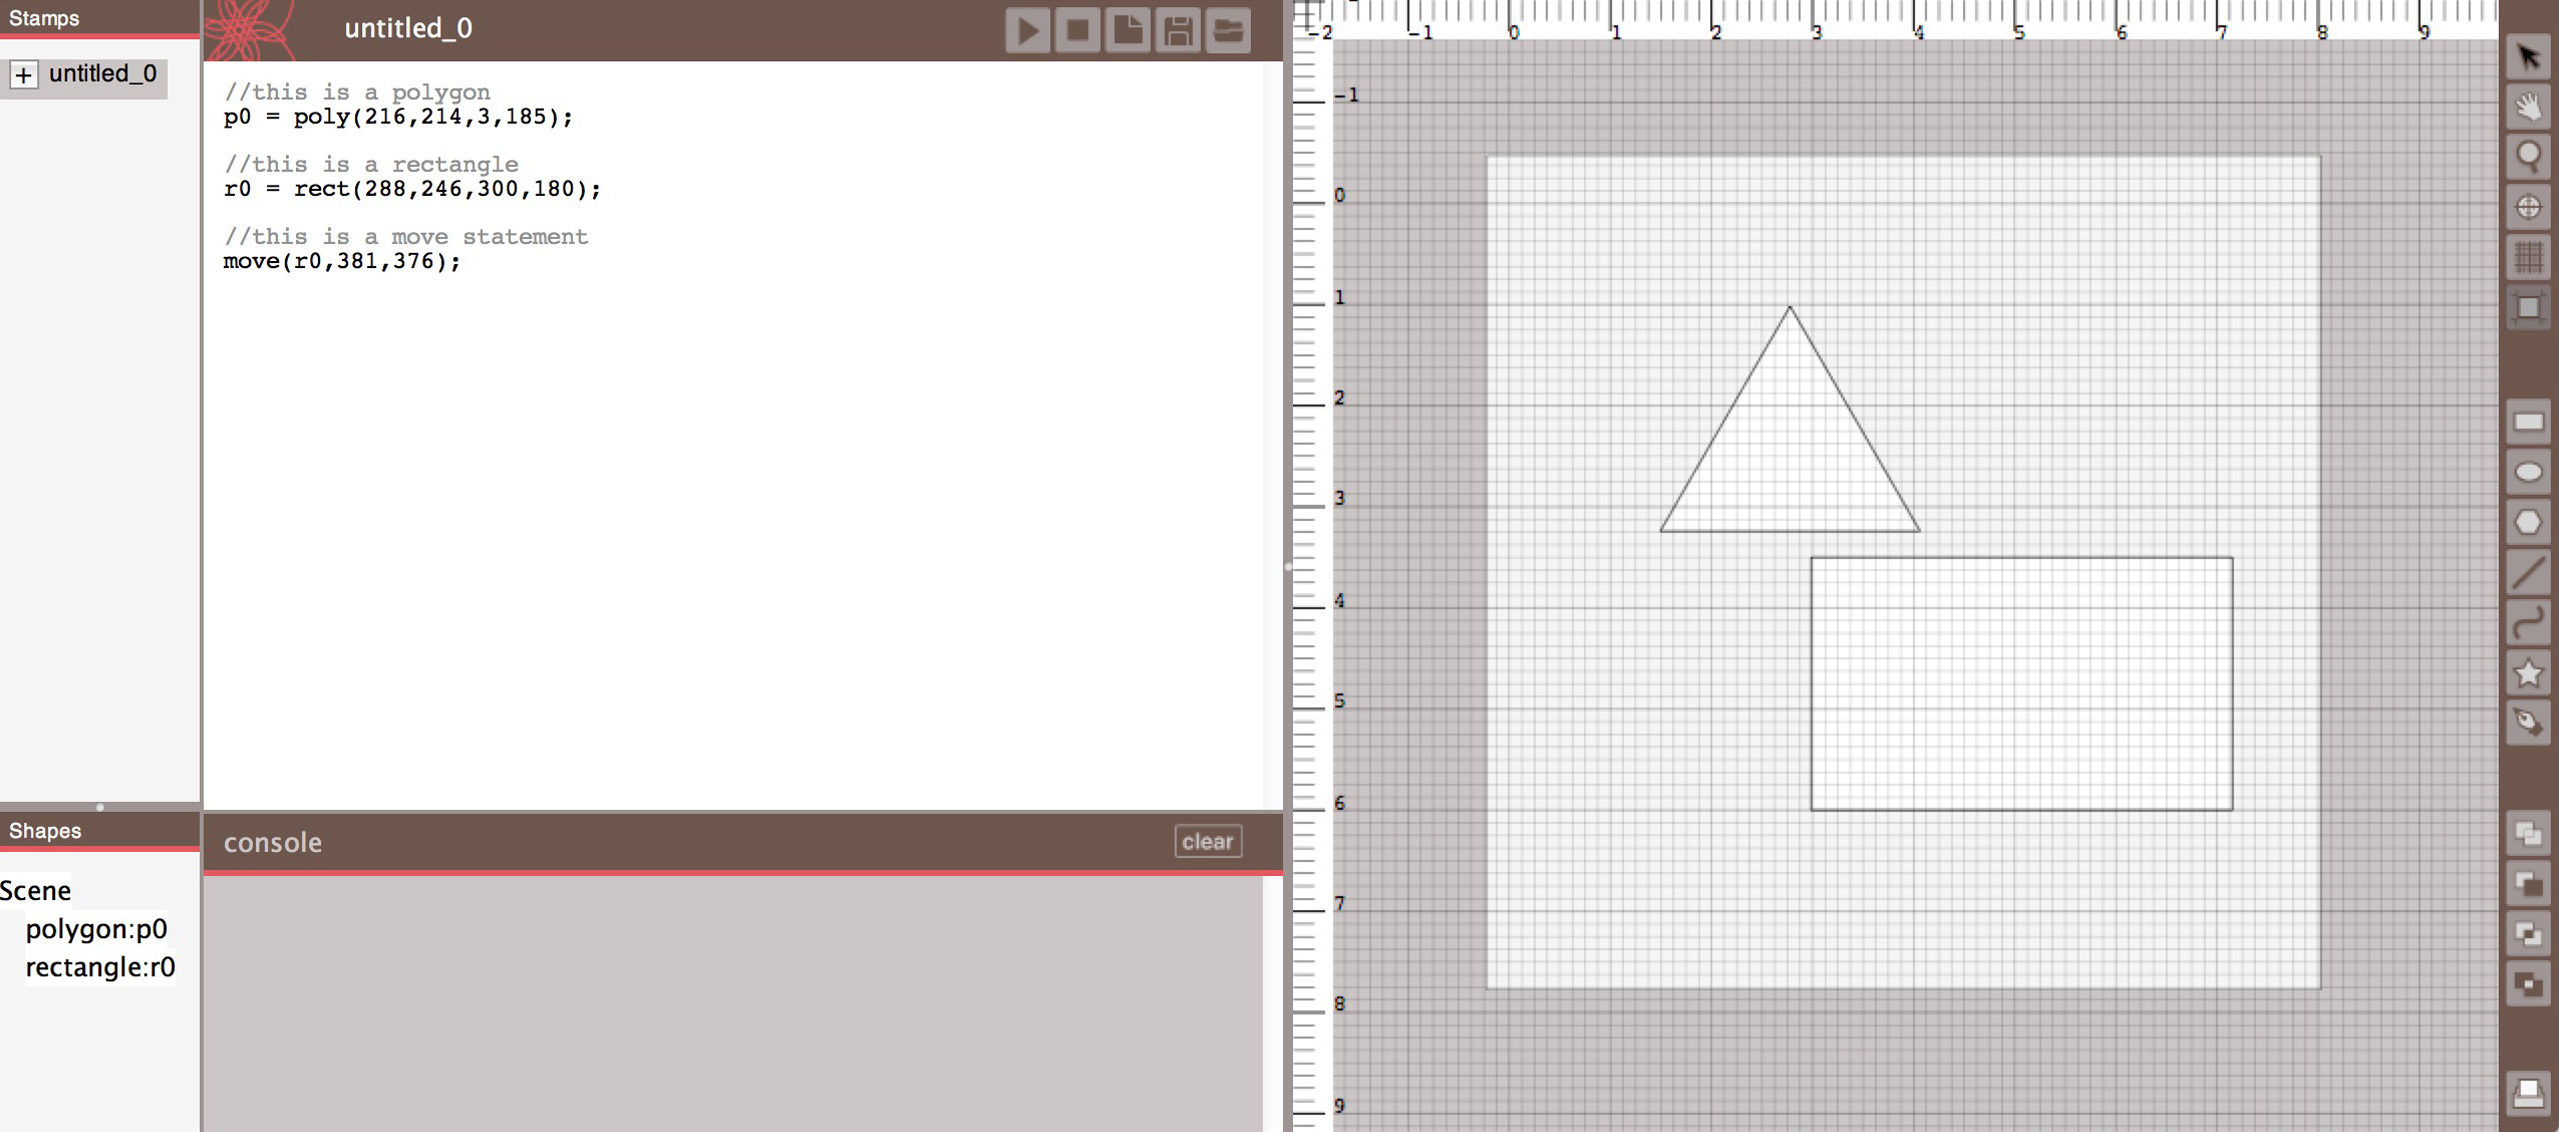
\includegraphics[width=0.75\textwidth]{images/application_image_sm_content.jpg}
\caption{The DressCode Software}
\label{fig:application_image}
\end{center}
\end{figure*}

\section{Related Work}
In the development of DressCode, we examined several fields of related software tools including learning-oriented programing environments, Computer Aided Design (CAD) tools with computational design functionality, and digital-design tools with linked forms of editing. Moreover, we situated our development of DressCode within the context of prior research in combining craft and computational design for young people.

\subsection{Learning Oriented Programing Environments}
 DressCode was developed to help young people use linked representations in the design of physical artifacts which distinguishes it from other novice programing tools. Logo is the seminal novice programming language founded on principles of constructionism and embodiment \cite{papert}. Scratch, developed in part as a successor to Logo, is one of the most actively-used novice-oriented programming environments, enabling children to create interactive screen-based media by combining command blocks \cite{resnick2}. Processing is a popular text-based programing environment environment developed to support artists and designers to creating complex forms and animations \cite{processing}. Logo, Scratch or Processing all contain a simplified programming syntax and prioritize visual applications. We chose to develop a new tool because we were interested in exploring the paradigm of linked representations, which neither Processing, Scratch or Logo were developed to support. It was easier to build our own software than to attempt to alter these existing platforms.

\subsection{CAD tools with Computational Design Functionality} 
Although computational design often is performed with general purpose programing languages and environments \cite{reas}, professional CAD tools have been developed that directly support computational design. Adobe software like Photoshop and Illustrator and 3D modeling tools such as Maya and Blender feature the ability to script behaviors in languages that are syntactically similar to Javascript, Perl and Python, respectively, however in these examples the programming interface is omitted from the primary interface. Other CAD tools emphasize programing. Grasshopper is data-flow programming environment that enables designers to combine visual modules and blocks to create 3D models in Rhino \cite{grasshopper}. DesignScript is an add-on to the Autodesk AutoCad software with an ever-present text editor, allowing users to script 3D forms through a combination of associative and imperative programing paradigms \cite{DesignScript}. OpenSCAD is a constructive solid-geometry modeling tool, where designs are created through textual scripts \cite{openScad}. Although these examples are powerful design tools, we argue they are not suitable for novices.

Novice-oriented CAD tools with computational design features are rarer than professional tools. FlatCAD is a domain-specific tool allows users to design customized gear-based construction kits by programming in FlatLang, a novice-oriented programming language modeled on Logo. and only supports design through text based programing \cite{flatcad}. TinkerCad is an entry level 3D-modeling tool for 3D printing. TinkerCAD includes "shape scripts": Javascript programs that produce 3D forms \cite{tinkercad}. Autodesk's 123D tools consist of a variety of novice oriented CAD applications that support the creation of designs for digital fabriation \cite{123D}, but only minimally enable computational design by allowing automated repetition of elements in predefined patterns. TinkerCAD and 123D emphasize physical creation, however their computational features are de-emphasized in comparison to their graphic design methods.

\subsection{Linked Editors}
Educational researchers have found when applied to the appropriate context, multiple external representations can reduce the amount of cognitive effort required to solve a problem, and often better communicate complex content \cite{ainsworth}. Linked representations have been primarily been applied to digital design tools in interface-design domains. Avrahami, Brooks and Brown demonstrated an early approach to a two-view system for designing user interfaces by combining a graphic editor linked with a special-purpose programming language \cite{two_view_ui}. Commercially, the two-view approach has been incorporated into web editors and GUI design tools in software development kits \cite{view_based}. Victor has advocated for the incorporation of linked representations in other fields including circuit design, game development and graphic design \cite{victor}. We seek to apply linked representations to a new context of entry-level physical computational design.

\subsection{Craft and Computing Research}
Eisenberg and Buechley's research on pervasive fabrication provides a survey of approaches and benefits in combining computational design and physical making for young people. Their research encompasses techniques and approaches for incorporating digital fabrication into educational settings, and describes how computational forms realized through digital fabrication enable youth to decorate their environments, allows them to create novel artifacts in the service of personal expression \cite{pervasive_fab}. Jacobs and Buechley engaged children in computational design through the use of Codeable Objects, a Processing library used to facilitate fashion design workshops \cite{codeable_objects}. Whereas Buechley and Jacobs re-purposed existing tools, we seek to develop a novel stand-alone tool to address difficulties experienced by novices using Processing: learning programing syntax, frustration with the lack of visual feedback, and the need for frequent instructor assistance in programing. 

\section{Dress Code Software Description}
DressCode is a 2D vector-graphic computational design tool that we developed for craft applications. DressCode supports \emph{linked editable representations} of a design in two forms: programmatic and graphic. Here we describe the interface and tool set of DressCode and the interactions between the programing and graphic components.

\subsection{System Overview}
The DressCode interface is divided into two primary panels: a graphic panel on the right and a text editor panel on the left (figure:\ref{fig:application_image}). A designer may write and execute programs using the text editor or they can draw and transform shapes using the mouse in the graphic panel. Each panel contains specific features and tools to enable these respective interactions. The text editor contains a console for output and error messages and a panel with buttons for compiling and running the current program. The design panel contains a re-sizable drawing board and grid with rulers and pan and zoom tools. A toolbar in the graphic panel contains a menu of drawing and transformation tools and a print button which allows the designer to export their design in vector format for output through printing or 2-axis forms of digital fabrication (figure:\ref{fig:graphic_tools}). The DressCode programming language functions via an interpreter with semantic functionality that we wrote using a Java-based parser-generator. The vector graphics consist of points, lines, bezier curves and polygons, and are rendered through a Java OpenGL wrapper. 


\begin{center}
\begin{figure}[h!]

\includegraphics[width=\columnwidth]{images/graphic_tools.jpg}
\caption{The graphic drawing and transformation tools in DressCode (from left to right: selection and move tool, rectangle tool, ellipse tool, regular polygon tool, line tool, curve tool, SVG import tool, pen tool)}
\label{fig:graphic_tools}
\end{figure}
\end{center}
\vspace{-20pt}

The graphic drawing tools include regular shape creation tools and a pen tool which enables free-hand drawing. The selection tool allows for individual shapes to be manually selected and moved, and the boolean operation tools allow for the combination of two or more shapes into a unified form through polygon-boolean operators (union, difference, intersection and either/or). The interface also contains two additional panels, the stamp panel and the declarative view which are described in following subsections.

We designed a custom imperative programing language for DressCode, which supports conventional programming data-types, loops, conditional expressions and user-defined functions. Variables in DressCode are dynamically typed. The language contains a subset of expressions which facilitate the drawing and transformation of 2D graphic geometric forms \textcolor{red}{add figure here to show syntax}. The language also supports math expressions and a variety of random noise generation methods. A note on terminology: for the remainder of the paper, we denote actions made in the graphic panel with the mouse as \textit{graphic actions}, and actions made in the programing panel by typing expressions as \textit{programmatic actions}. We also distinguish between two types of actions: \textit{initialization actions} denote programmatic or graphic actions which result in the creation of a new shape and \textit{transformation actions} denote programmatic or graphic actions which result in an existing shape being moved, rotated, scaled or otherwise altered.


\subsection{Linked Representations In Practice}
We developed the linked representations in DressCode around two primary design principles: correspondence and readability. We describe the latest state of the tool with respect to these principles. We wish to emphasize however, that this state was achieved though a series of tests with successive versions in our workshops.

\subsection{Correspondence}
\label{subsec:correspondence}
The governing design principle in DressCode is correspondence between programmatic actions and graphic actions. For every shape that is initialized programmatically, a shape is generated in the graphic view. Conversely, for each graphic action, a corresponding programing expression appears in the text editor. We designed the DressCode programing language to support the translation between graphic and programmatic representations. The drawing API is formulated on an Object Oriented Programming paradigm where basic shapes (points, lines, curves, polygons etc.) are initialized by calling the appropriate method and passing it a set of parameters designating its location and dimensions. If a shape is initialized graphically, its parameters are determined by the mouse gestures of the designer (where they click to determine the origin, and how far they drag from the origin to determine the dimensions). The method-type of the auto-generated expression that results from a graphic action is determined by the type of graphic tool that was used to create the shape.

Transformations, including moving, scaling, rotation, color and stroke changes, and shape booleans follow a similar structure to shape initialization. In the programing language, transformations are performed by either wrapping a shape-initialization expression in a transformation expression, or by assigning an identifier to the shape, and then calling the transformation method with the identifier. On the graphic side, each transformation tool corresponds to a transformation method in the DressCode language, enabling the generation of a corresponding expression in the programing panel which contains as its first argument a reference to the shape which was selected and manipulated graphically. Throughout the design process, a complete representation of the current state of the graphic design is continually maintained in the programming panel.

\subsubsection{Static and Dynamic Generativity}
Generativity is one of the most powerful aspects of computational design, but its systematic nature is less easily represented in graphic form. DressCode contains functionality persevere correspondence while maintaining useful and flexible representations of random distributions. to help people organize their code in the form of \textit{stamps}: graphically created functions that return shape primitives. Static stamps translate an instance of a design generated by random programmatic methods to a set of statements that describe discrete shapes with hard-coded parameters. This enables users to programatically represent specific instances of a generative design (see Figure \ref{fig:stamps}). Static stamps are created by graphically selecting a single primitive or group with either the selection tool or the declarative view, and selecting the static stamp option. Stamps are listed in the stamp menu and can be added to a user's primary program by selecting the \textit{+} icon next to each stamp. The code of a stamp can be modified by the user after it is generated. This representation allows multiple versions of a generative pattern to be preserved in a single design, and enables specific patterns programs to be shared and remixed. If the textual program from one design is copied and inserted into another designers program, it will re-generate the exact design in the context of the new design.

\begin{center}
\begin{figure}[h!]
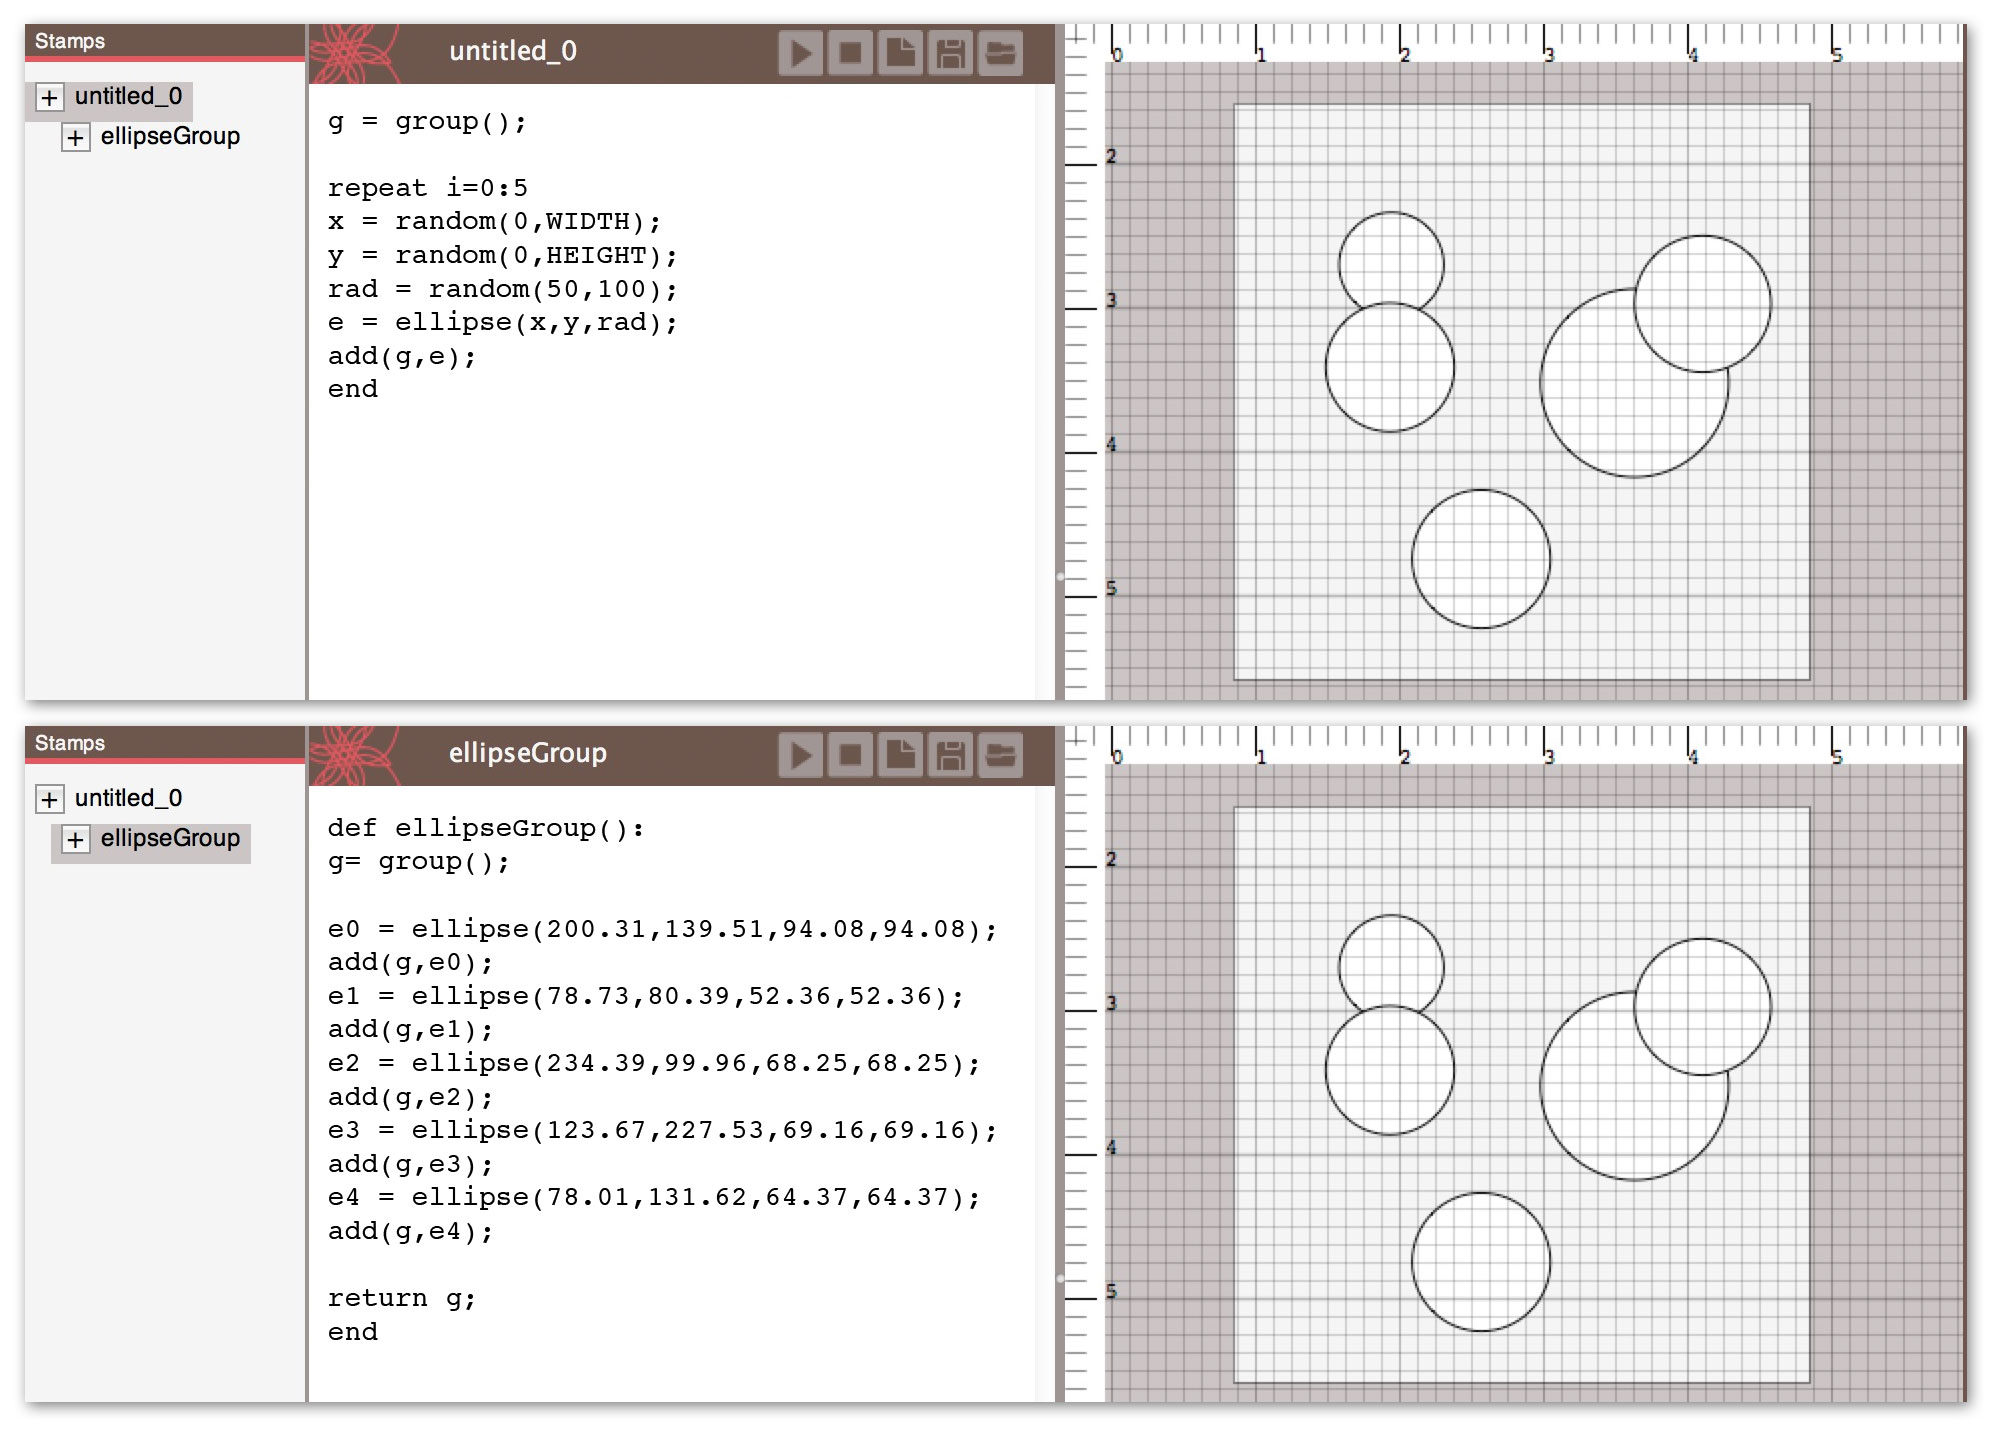
\includegraphics[width=\columnwidth]{images/stamps.jpg}
\caption{Static stamp functionality. (Top: User defined code which generates five random ellipses. The ellipses' positioning and size will change each time the program is run. Bottom: static stamp created from ellipses which will always return the same design.)}
\label{fig:stamps}
\end{figure}
\end{center}
\vspace{-20pt}

\subsection{Readability}
\label{subsec:readability}
As we discovered through our implementation, Symmetry between graphic manipulation and textual programing must be tempered by concerns of usability. Merely producing a textual expression that accurately reflects a graphic action does not ensure that the interaction will be interpretable to the designer, let alone useful. We considered how we could design linkages between programmatic and graphic actions which were not only functional, but transparent, readable, and reconfigurable by young people. 

\subsubsection{Readable References}
Like many existing programing languages, DressCode gives the developer flexibility in how elements are referenced. Because the DressCode language enables methods to be nested within one-another, there is a degree of ambiguity for how identifiers can be used. In creating the linkages, we considered \textit{how} shapes should be referenced when transitioning between programmatic and graphic representations in a way that was readable. 

All initialization graphic actions produce programmatic expressions that are automatically assigned an identifier. Subsequent transformation graphic actions will produce programmatic expressions that reference the auto generated identifier on the following line. This produces code that while requiring more lines, is arguably more readable than a nested chain of expressions. If a shape that was programatically initialized without an identifier is transformed graphically, DressCode will recognize the distinction and resort to wrapping the initialization expression in the appropriate transformation expression. If the designer re-assigns or modifies the identifier of a shape through a programmatic action, future graphic actions on the shape will recognize this and use the new identifier.

\subsubsection{Readable Edits}
It was also important to consider where auto-generated expressions would appear within a program. For an initialization graphic action the programming expression will always appear below the last line in the program. If the designer performs a transformation graphic action however, the expression will be inserted into the line below the initialization of the selected shape, or below the last transformation expression for the shape. This structure ensures that the modified program will reproduce the correct order of operations when run, but also provides a form of organization to auto-generated statements. 

This structure also enables an auto-generated program to demonstrate steps used to arrive at a design. Because the DressCode programing language employs an imperative paradigm, designs are represented as a series of the designer's actions, rather than a declarative state. We structured the auto-generated statements so that the programmatic expressions reflected the order of steps a designer made in the graphic interface. For example, when a shape is moved with the move tool, a textual move expression is inserted into the designer's program. For all subsequent moves following the first move, rather than generate a successive string of additional move statements, the move expression is updated to reflect the new coordinates of the shape. However, if another tool is used to alter the shape, or a programmatic expression is manually inserted by the designer following the move statement, future actions with the move tool on the same shape will generate a new move statement, which will be subsequently updated until another tool is used (see Figure \ref{fig:auto_generated_code}). This same logic applies to all other transformation tools.

Naturally, in manually writing code, the designer may deviates from this organization. Fortunately, manual edits will not prevent the ordering mechanism from functioning for successive graphic actions. Furthermore, the consistent, simple rule-set for auto-insertion enables the designer to anticipate where expressions will be inserted into their code, and distill the steps they took to arrive at a design, both which we believe facilitate understanding the program, and making future edits.

\subsubsection{Tree Representation}
As programs grow in length and complexity, it is helpful to provide other representations that may make the structural relationships in one's code more readable. Many professional code editors contain tree-views of all of the methods and identifiers in a class, providing an alternative means of navigating one's code. We combined these tools in a way that is specific to graphic computational design. DressCode features a tree view which contains a listing of all groups of shapes in the current design. Child shapes are nested within their parent groups. When selected in the tree view, the shape is selected and highlighted in the design view, and the line where the primitive was last modified in the text-editor is highlighted (see Figure \ref{fig:declarative_view}). The tree view provides visual feedback on how elements of a design connect to the program, and provide a practical selection technique for complex designs.

\begin{center}
\begin{figure}[h!]
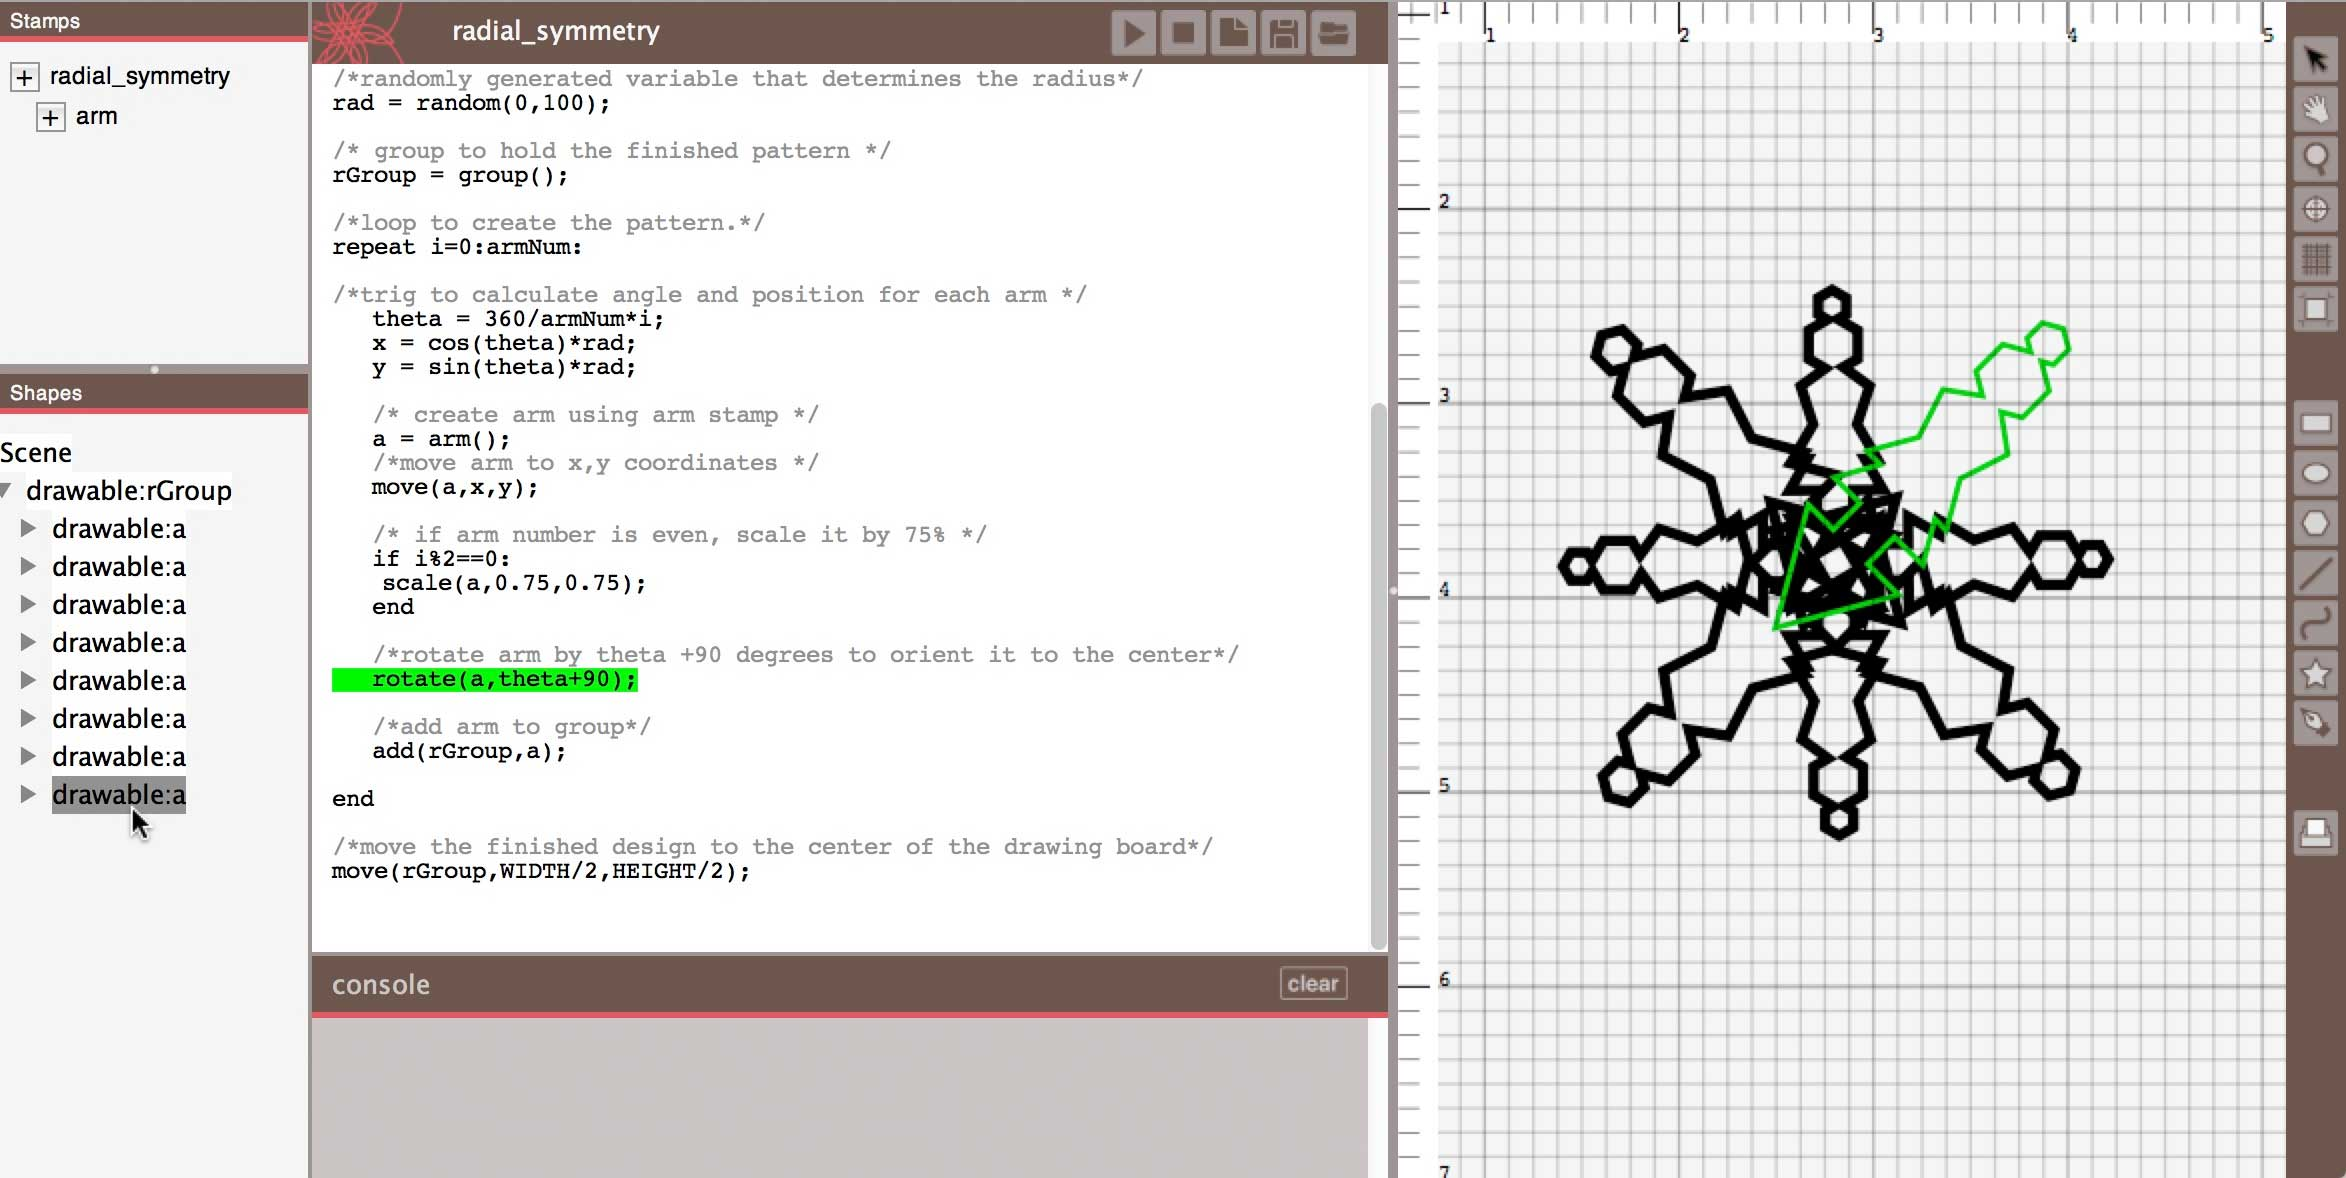
\includegraphics[width=\columnwidth]{images/selection_mechanism.jpg}
\caption{Declarative view with selected primitive}
\label{fig:declarative_view}
\end{figure}
\end{center}
\vspace{-20pt}

\section{Workshops}
We evaluated DressCode with young people through two workshops with young people. The preliminary workshop consisted of a one-day session in which participants designed and fabricated leather wrist-cuffs with a preliminary version of DressCode. Following this workshop, we revised the software and conducted a long-term evaluation through a four-day workshop in which participants created computational designs with the current version of DressCode and screen-printed them onto t-shirts. The workshops were designed to help us evaluate how the linked representations in DressCode could be applied in realistic contexts for the production of finished artifacts. We focused on three primary criteria for our evaluation:
\begin{itemize}
\item Accessibility: Was DressCode accessible for novice use, and what types of design practices did it foster?
\item Relevance: How did the use of DressCode in the context of craft applications connect with the existing goals and interests of the people who worked with it?
\item Diversity: Did the workshops result in a wide range of design approaches and end artifacts?
\end{itemize}

\subsection{Evaluation Methods}
The participants' experiences were evaluated through written surveys, interviews and group discussions. The surveys were aimed at understanding participants’ prior attitudes towards programming, design and craft, their interest in and attitudes toward programming and design, and their engagement in and enjoyment of the workshops. In-person interviews were conducted with the participants in the preliminary workshop. In the primary study, participants were engaged in three group discussions at the start, middle and end of the workshop.

\subsection{Preliminary Workshop: Wrist cuffs}
The preliminary workshop was conducted among 10 young adults, aged 15-17, two male and eight female. Of those surveyed, three participants had prior experience with Scratch, and two had worked briefly with the Arduino programming environment in a prior workshop. All participants said they had some prior experience in art, design, or craft. Prior to the workshop, 60\% of the participants indicated that they did not feel comfortable programming on their own; however, the majority indicated they were interested in learning more about the process. The preliminary version of DressCode used by participants featured the current version of the programing language, and a linked graphic move tool, but no graphic drawing tools.

During the workshop, participants used DressCode to design a pattern for a wrist cuff, laser-cut their patterns into leather and assembled the finished wrist cuff by hand. The computational design in the preliminary study was structured around radial symmetry, and the majority of the resulting artifacts featured patterns that were derived from radially symmetric structures. Participants wrote their own radial symmetry algorithms and were then provided with a template in DressCode that automatically clipped their designs to the dimensions of a cuff sized to their wrist. By the completion of the workshop, each person had designed, cut and finished their own wrist cuff.

\subsection{Preliminary Results}
 While each wrist cuff was unique, the aesthetic variation of the finished artifacts was not as strong as we hoped. Most people liked the finished artifacts; eight of the participants said they planned to wear the bracelets they created, and two planned to give them as gifts. It was evident that the female participants were more excited with the end artifacts then the men. A comparison of the pre and post surveys demonstrated increased comfort with programming as a result of the activity. All participants stated that they believed they could use programming to make things that were beautiful, whereas several had disagreed with this statement before the workshop. All participants unanimously identified the programing portion as the most difficult component of the workshop, however the majority said they were interested in continuing to learn more about computational design for craft applications. We also had many requests for a better means of saving "in progress versions" of designs. 

\subsection{Design Revisions} Following the preliminary workshop, we extended the linked representations in DressCode to include graphic drawing tools, and additional graphic manipulation tools. We also updated the look and feel of the interface and added the tree view and stamp tool. We were dissatisfied with the limited manual engagement of crafting leather bracelets (most of it was done by the laser cutter), and we also recognized that it could be alienating to some people. We shifted the focus of the next workshop to design for screen printing t-shirts.

\subsection{Primary Study: Screen Printing}
The screen printing workshop was conducted among 7 young adults, aged 13-17, and one older participant, aged 21. Three participants were male, and five were female. Participants were selected to represent a range of programming, craft and design experience (table \ref{table:experience}).
\begin{table}
 \centering
 \begin{tabular}{|c|c|c|c|c|c|}
  \hline
  \multicolumn{1}{|p{0.75cm}|}{\centering\tabhead{}} &
  \multicolumn{1}{|p{1.3cm}|}{\centering\small{no experience (1)}} &
  \multicolumn{1}{|p{0.75cm}|}{\centering\small{2}}&
  \multicolumn{1}{|p{0.75cm}|}{\centering\small{3}}&
  \multicolumn{1}{|p{0.75cm}|}{\centering\small{4}}&
  \multicolumn{1}{|p{0.75cm}|}{\centering\small{expert (5)}}\\
  \hline
  \small{art} & 0 & 0 & 4 & 4 & 0\\
  \hline
  \small{craft} & 1 & 0 & 3 & 4& 0 \\
  \hline
 \small{programming} & 1 & 1 & 4 & 1& 1 \\
  \hline
 \small{design} & 0 & 2 & 3 & 3& 0 \\
  \hline
 \end{tabular}
 \caption{Prior participant experience. (Numerical values in the columns correspond to the number of participants with that response.)}
\label{table:experience}
\end{table}
\subsection{Workshop Progression}
Prior to the workshop, we had participants select t-shirts in a size and color of their preference. Participants were given the task of creating a computational design to screen print onto a t-shirt they would want to wear. We introduced participants to DressCode, focusing on principles of generative design and the use of random noise. In the process, we provided them with a set of example designs that showcased different computational techniques like random-walks, clipping masks and gaussian distributions. We also demonstrated the process of photo-emulsion screen printing and had participants stretch and prepare their own screens. Following a series of iterative critiques and design sessions where participants made revisions to their designs, participants printed out their final designs on transparencies, transfered them to their screens through an exposure process and printed onto their shirts (see Figure \ref{fig:screen_printing_process}).
\begin{center}
\begin{figure}[h!]
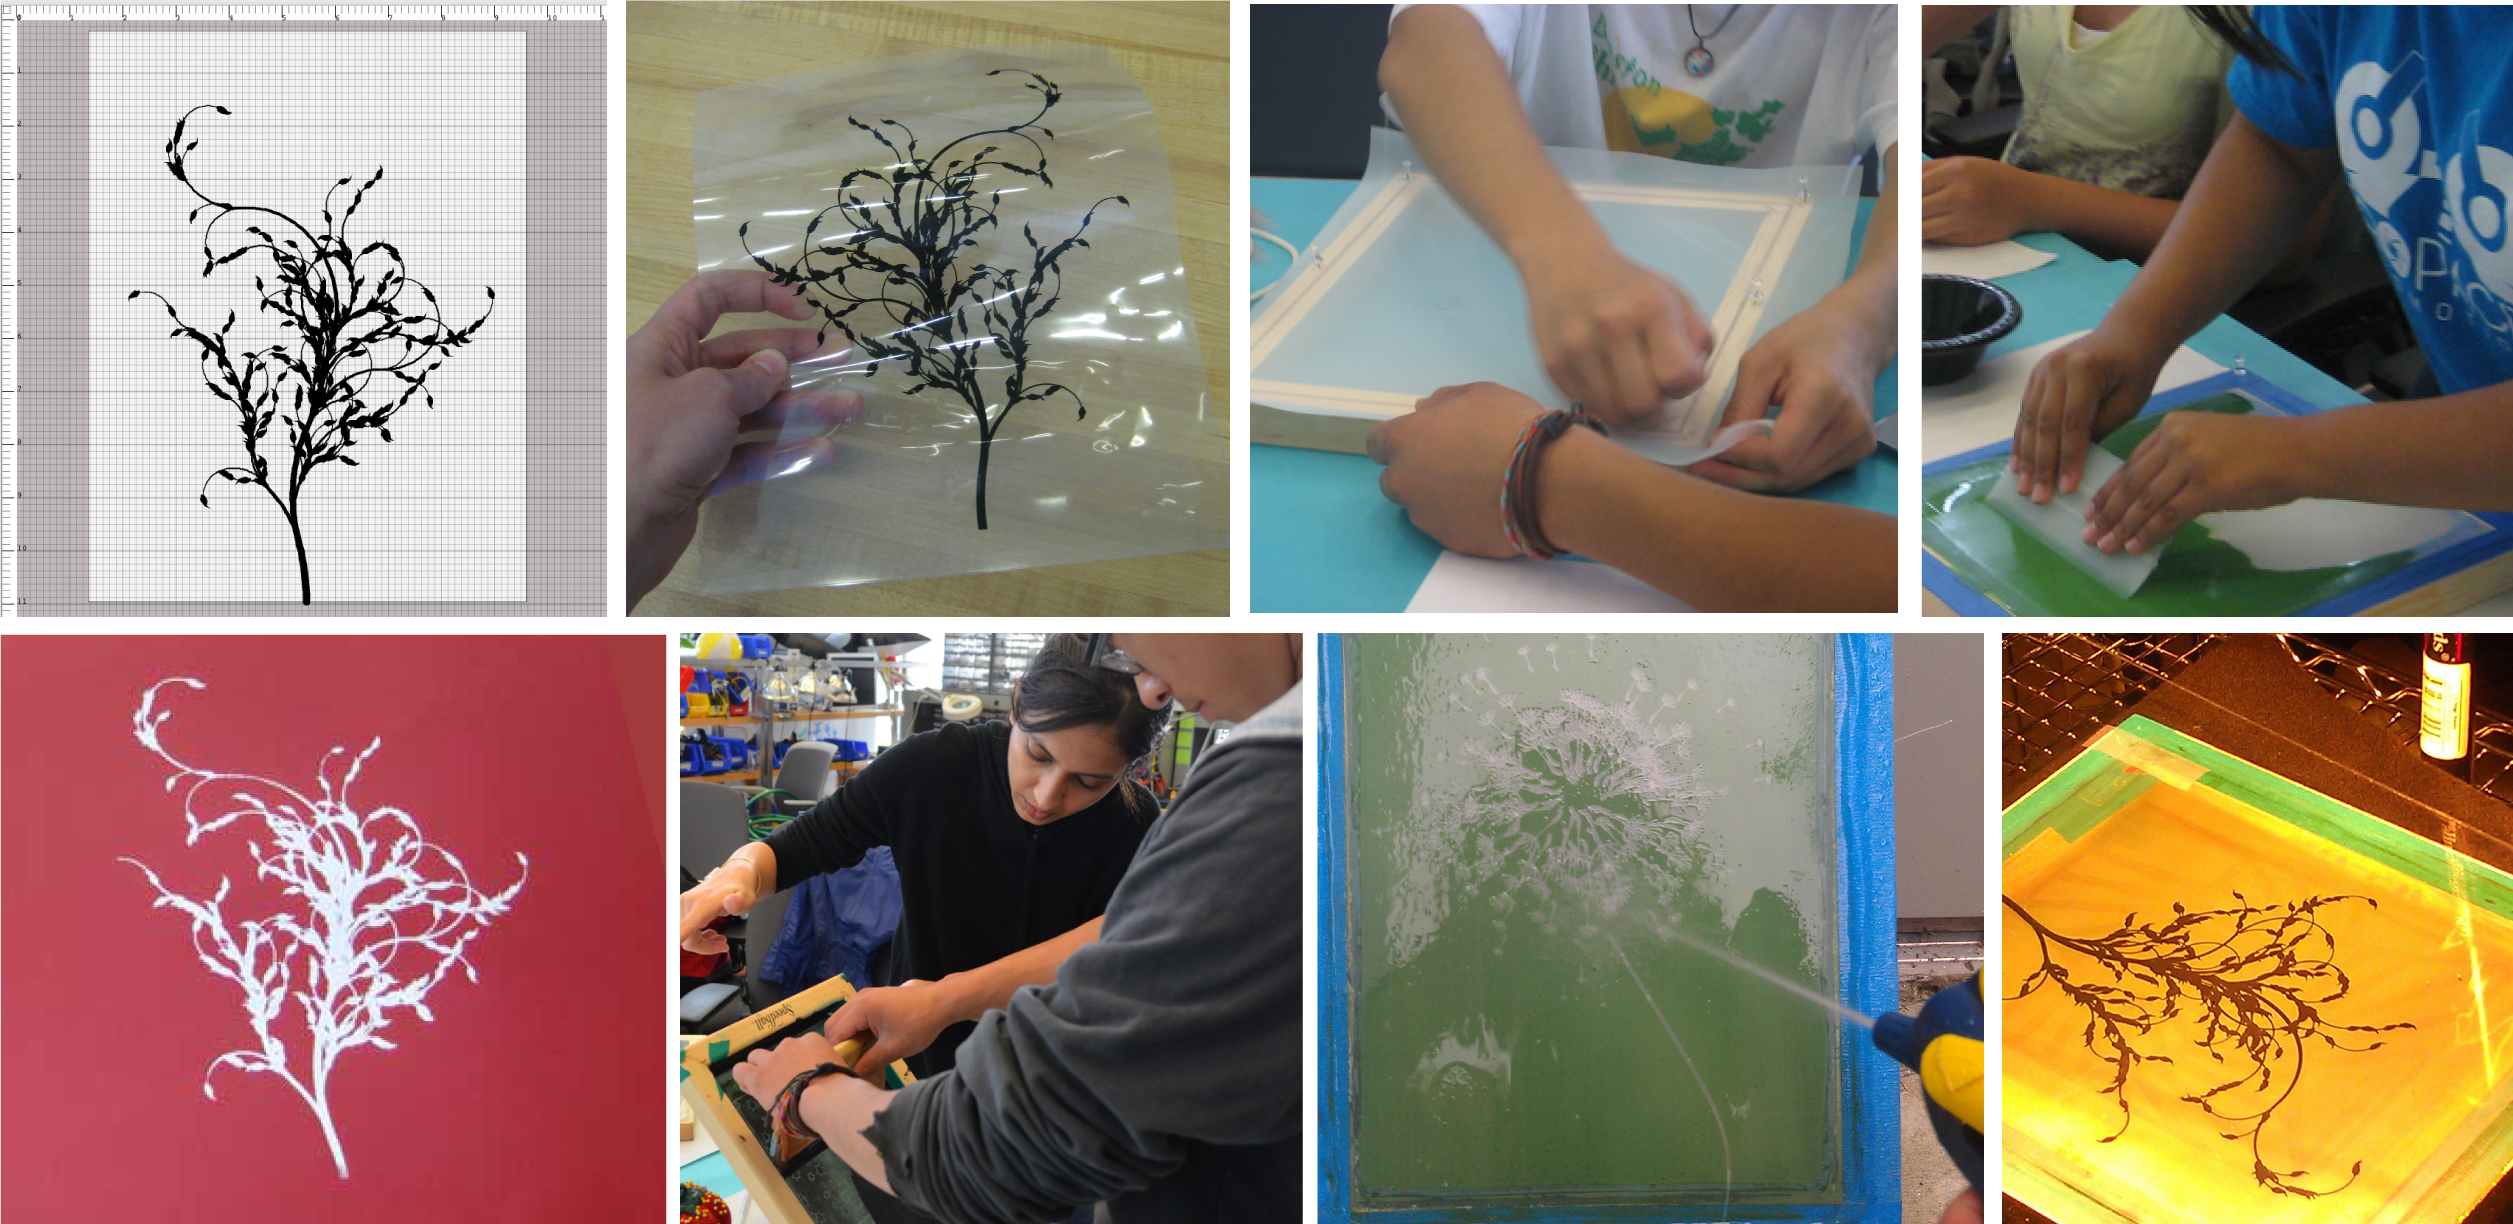
\includegraphics[width=\columnwidth]{images/screen_printing_process.png}
\caption{Screen printing process. (Clockwise from upper-left: Digital design, printed transparency of design, stretching the screen, applying photo emulsion, exposing the screen with the transparency, washing out the screen to reveal the design, printing with the finished screen, a completed print.) }
\label{fig:screen_printing_process}
\end{figure}
\end{center}
\vspace{-20pt}

\subsection{Screen Printing Results}
The screen printing workshop was extremely popular. Each participant in the workshop was successfully able to use DressCode to produce a design for their t-shirt (see Figure \ref{fig:screen_results}) which they planned to wear. Two participants not only printed to the provided shirts, but also brought in additional garments to print on for friends and family, and all requested to keep their screens following the workshop, and stated on the that they planned to continue making prints for themselves and others. Two participants contacted us via email following the workshop thanking us for the experience, and requesting tips on how to properly care for their garments, and requested to be included in future DressCode activities. 

In the screen printing workshop, we observed three general design approaches: 1) emphasis on programmatic methods: participants who used the graphic drawing minimally, almost exclusively relying on generating and transforming methods computationally. All of the participants in the first workshop fit this category (due to the lack of extensive graphic drawing tools), as well as three of the participants in the screen printing workshop. 2) Programmatic manipulation of provided graphic elements: two people in the screen printing workshop used programming expressions to manipulate pre-existing graphics that had been provided in examples. 3) Equal use of graphic drawing and programmatic manipulation: Three people in the screen printing workshop used the graphic drawing and transformation tools in equal proportion with programmatic methods.

\begin{center}
\begin{figure}[h!]
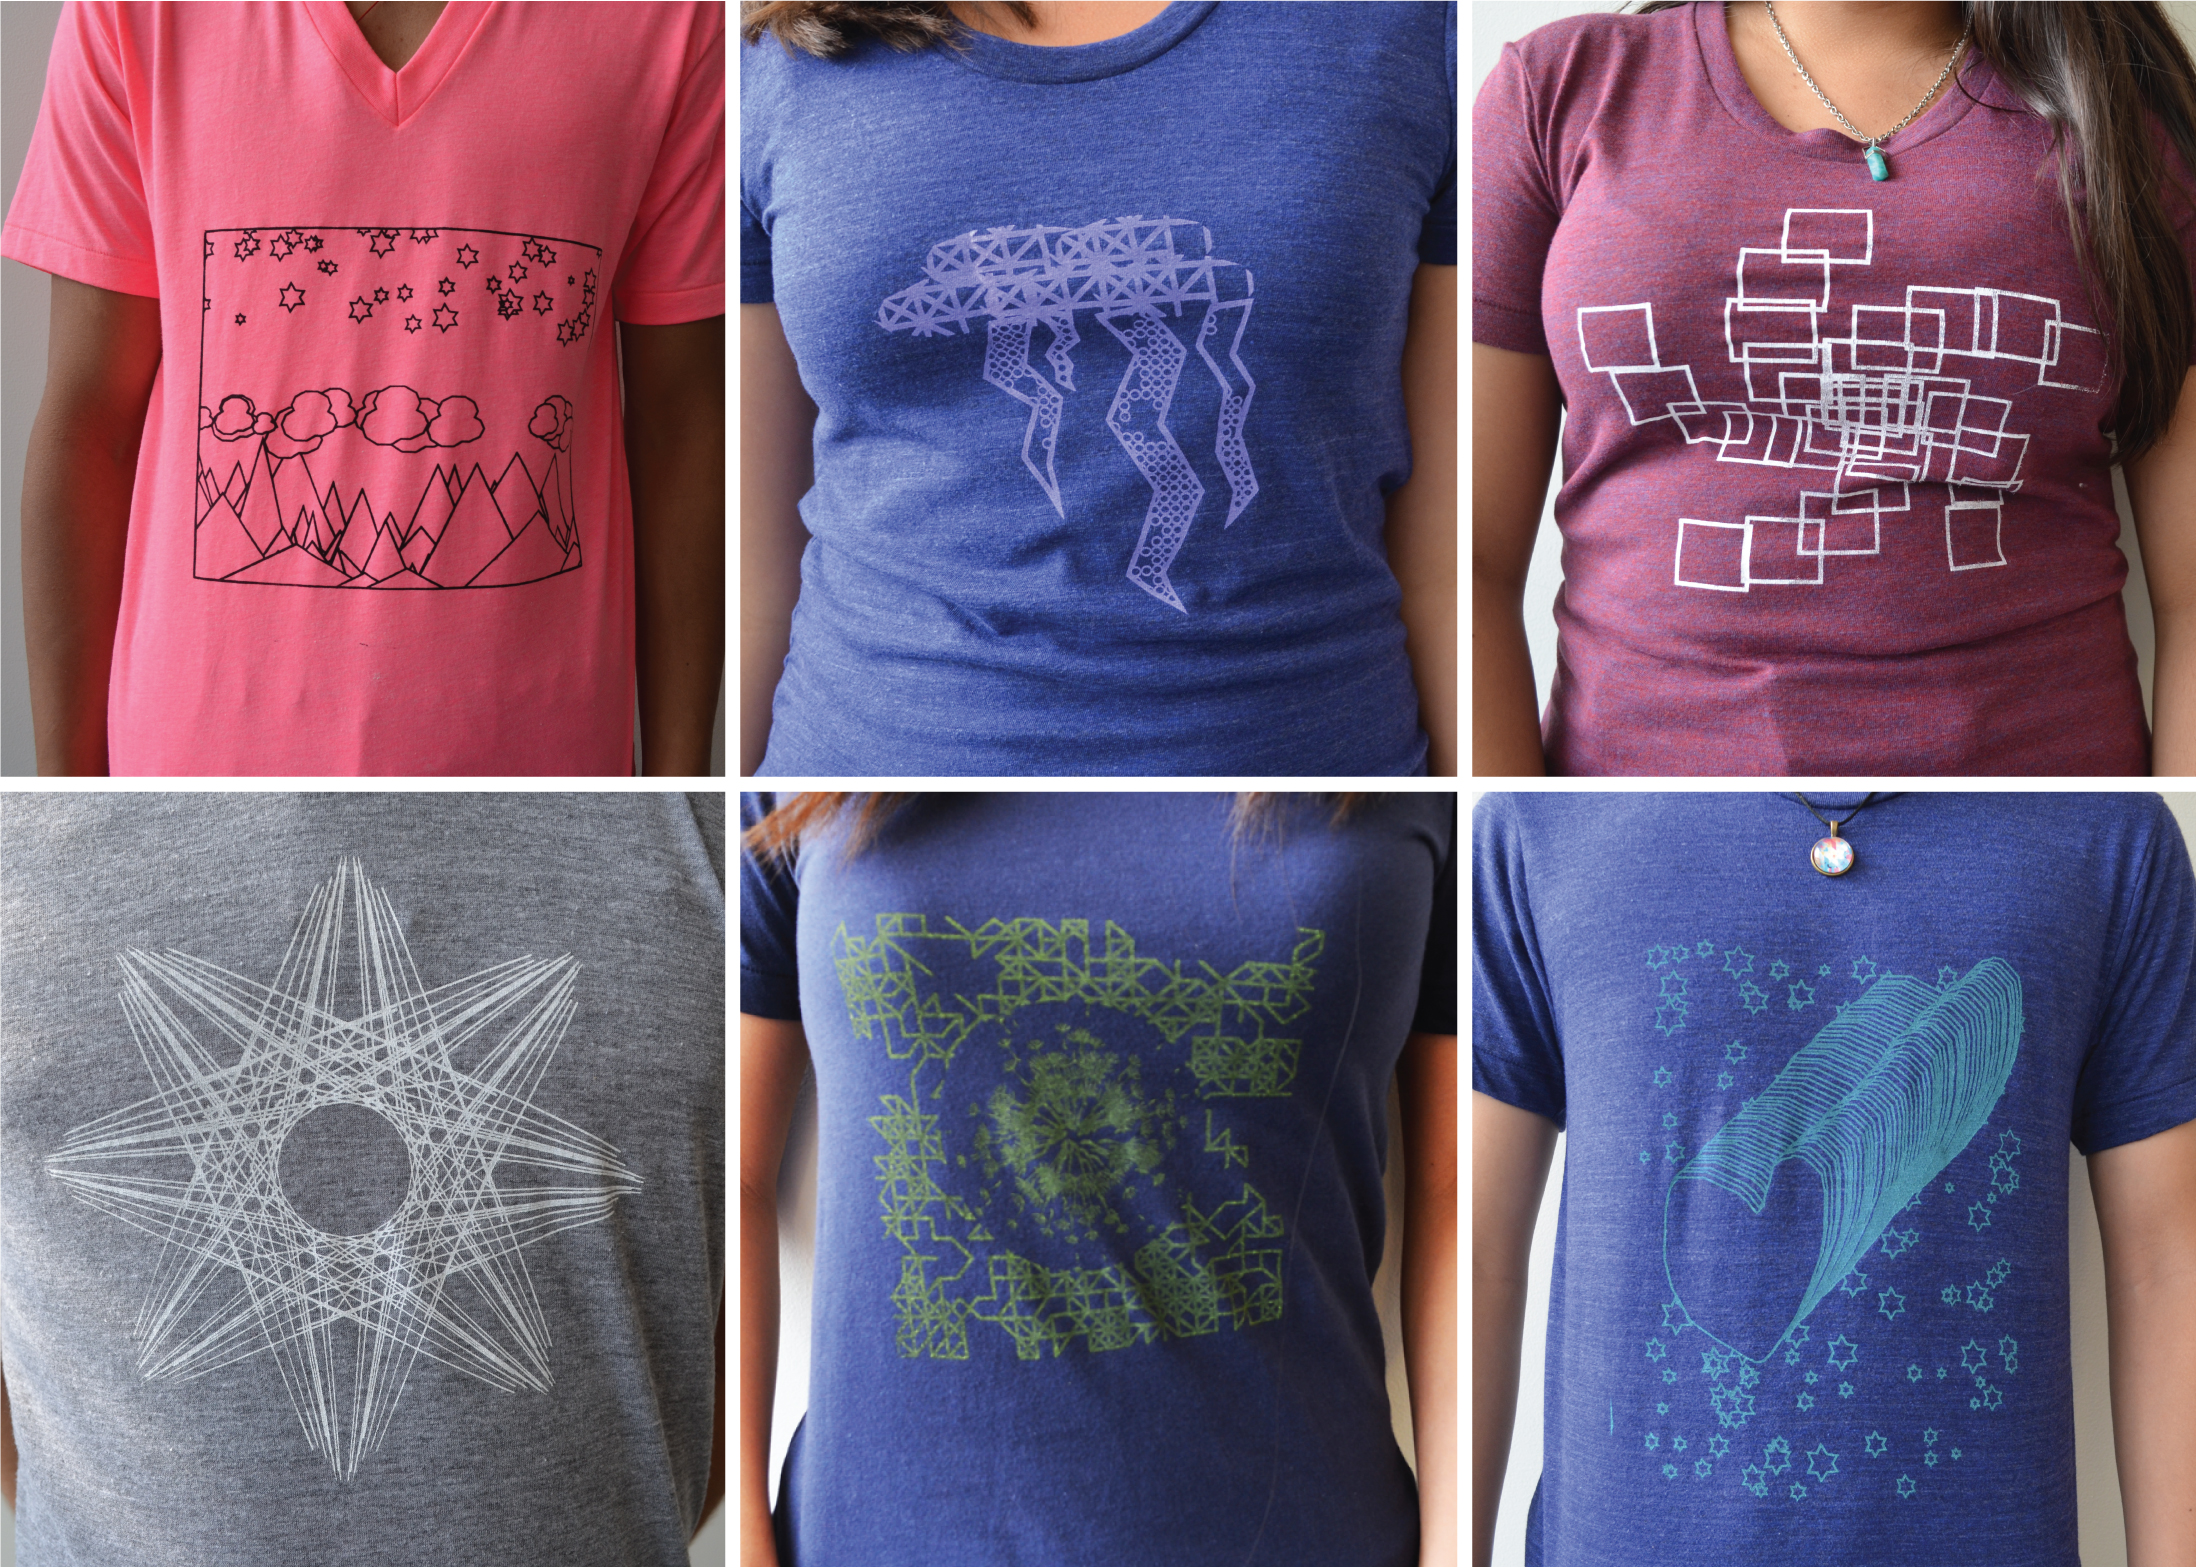
\includegraphics[width=\columnwidth]{images/shirt_results.jpg}
\caption{Some of the completed shirts. (Clockwise from upper-left: generative landscape, clipping mask cloud pattern, geometric spiral, random walk of hand-drawn hearts, dandelion-random walk mashup, generative linear-radial pattern.) }
\label{fig:screen_results}
\end{figure}
\end{center}
\vspace{-20pt}

Participants attitudes towards programming changed from what they were after the computational design sessions. In the majority of cases, this change was positive; participants indicated greater interest in learning programming in the future, a stronger belief that programming was a tool that they could create things they would use in their daily life, and greater comfort in programming on their own following the craft activity. Participants were positive about the graphic tools, although they requested that their functionality be extended to incorporate a greater range of transformation methods. All participants said they would be interested in using DressCode for another activity, and all but one indicated they would like to continue using the programming language in particular.

\section{Discussion}
Reflecting on the experiences and comments of the people involved in our workshops, we discuss some of the broader implications of DressCode. We focus on reactions from the participants in the screen printing workshop as it constitutes our primary study of DressCode, but include reactions from the wrist cuff workshop to demonstrate distinctions in practice and attitudes between the two experiences. 

\subsection{Diversity in design practice}
We found that linked-representations in computational design tools leads to diversity of design practices for novices in three ways. The intuitive graphic tools offers a way to scaffold the process of learning programing. Enabling correspondence between graphic and programmatic manipulation provides flexibility in the degree to which people rely on computational or graphic methods, and that linked representations can foster noteworthy design aesthetics that blend qualities of hand drawing with computational complexity and repetition.

Responses from the screen printing participants demonstrated that the graphic portions of linked representations were easy for people to use. Before the graphic tools were demonstrated, several participants independently started experimenting with them and described their use to be self evident. Furthermore,the linkages between the graphic drawing and programing were described as being helpful in understanding the programing portion:
\begin{quote}
\textit{[Having a graphical side and having it auto-update the code, it can show you that [if] you want to work with the code you're learning as you're using the GUI. So that people could try and say ok, if I can't do something with the graphical tools, let me try and manipulate the code. And then you already have some understanding because you've been using the graphical tools and it's been appearing over there the entire time.}
\\Participant B
\end{quote} 

People also understood however that programing was well suited to tasks that would have been difficult to accomplish with graphic tools alone. One young man created a generative landscape with hand-drawn elements that were repeated in different positions. Because he structured the design as a parametric program, when he decided to alter the composition dimensions, he was able to avoid the task of manually re-positioning each element:
\begin{quotation}
  \textit{[DressCode] made changes much easier to change, rather than redoing the entire design}
  \\Participant R
\end{quotation}

The combination of graphic drawing and programing also resulted in aesthetics that we as computational designers found to be incredibly exciting. The participants who relied on a balance of graphic and programmatic design tools produced designs that contained imperfect, irregular forms in direct conjunction with computational order, repetition and complexity. These designs were distinct to the individual creator, and their imperfections were deliberate. During one critique session, the creator of the heart t-shirt explained that he had deliberately chosen to draw a irregular heart form, because that was "his style". That visual qualities of these hand-drawn/computational hybrids (to borrow a term from Zoran \cite{zoran_thesis}) demonstrate that computational tools can support evidence of the human hand rather than eliminating it. We consider the development of a more nuanced palette of hand-drawing graphic tools and mechanisms (perhaps a tablet and stylus), as a worthy next step of exploration in this field.

\subsection{Tensions in linked representations}
Computational tools for novices often abstract lower-level functionality to ensure ease of use. In the context of linked representations for computational design, abstractions between graphic actions and computational correspondence should be weighted with respect to the assumptions they make about the intentions of the designer, and their ability to effectively represent the powerful ideas behind programing for design.

People in the screen printing workshop had a range of opinions regarding what new graphic tools should be added to DressCode, how these tools should correspond with programing, and if existing features could represented graphically. Because most people used some form of randomness in their design, there was a debate on whether the creation of random distributions should be a graphic or programmatic. Two of the young women stated that they would have preferred graphic tools that enabled them create random groups of objects by pointing and clicking with the mouse. Another participant wanted the software to store the randomly created values for a specific program, and then have a graphic button that enabled him to reset these values to new random numbers. Still three others stated that they preferred creating random distributions using loops and variables in the text editor, and recognized that by creating random distributions graphically, DressCode would become too similar to existing tools, and lose some of the control gained through programing:
\begin{quote}
\textit{The important thing I really feel about DressCode is you can turn things like ''random". These are drawn [gesturing to a graphically drawn element of his design] and these are from the programing part [gesturing to the repetition of them] ... but in [Adobe] Illustrator it's just drawing. You can't have everything.}
\\Participant Z
\end{quote}

Similarly, participants had different ideas for how new graphic tools should generate programing statements. Here two people discuss their ideas for the incorporation of an eraser tool:
\begin{quote}
Participant Z (Talking about erasing graphically): \textit{So if you erase one line, it becomes two lines...so it's going to generate the code for two lines.}
Participant M: \textit{No like if you drew a line with the sidebar, and then you decided you didn't like, you don't have to go to the code, erase it and press play, you could just take the erase tool, click on it and then it goes away.}
Participant Z: \textit{No, what I mean is like if you just wanted to erase half..}
\end{quote}

In linked representations, defaulting to making every programmatic action represented by a graphic action can lead to the trivialization of the ideas behind programmatic forms of representation. Relegating random distributions to a pre-defined set of graphically selectable icons may make them more accessible for immediate use, but it could also prevent a designer from understanding the design potential of generativity. Furthermore, the automatic inclusion of features that seem simple (such as an eraser tool) may in fact lead to inaccurate assumptions about the design objectives of the people using the tool. In developing linked representations between programing and graphic interactions, we advocate the following approaches. One, incorporate graphic drawing tools that are intuitive and familiar, and can be directly linked to a single programing method. Two, developing novel solutions for programmatic structures that are difficult to represent graphically (for example our use of stamps to deal with the correspondence issues raised by randomness). Three, do not rely exclusively on graphic tool correspondence to support entry into programing, but instead incorporate other forms of visualization and representation (such as the tree view), to help people understand the relationships between the program and the graphic design.

\subsection{Designing experiences for diverse interests}
People approach tools and activities with different motivations, and their response to a tool will be prominently affected by how relevant the activity was to their subjective interests. In both the wrist-cuff and screen printing workshops, we observed great diversity in how people valued their experience. Several young people were concerned with producing things that were unique, or expressed their personal style:
\begin{quote}
\textit{You can't find it at American Eagle. I buy a lot of my bracelets there, and you can't just go there and find this. I think it's cool if someone were to say ''Oh where did you get that from?, You can't find it.".}
Participant C
\end{quote}
Whereas others were excited about the opportunity to program:
\begin{quote}
\textit{``[The] computer programming was enjoyable for me because I had wanted to do it before but never had the chance. So this workshop gave me exposure to something that I wanted to do for a while and I totally loved it."}
\\Youth Participant 092297m (survey)
\end{quote}
We also found that people valued the opportunity to learn a craft process:
\begin{quote}
\textit{When you're screen printing there's the manual labor involved, so when you actually get something right it's I guess more gratifying, since you put hard work into it... Well you do put hard work into programming, but it's more a thinking thing, not actual physical labor.}
Participant L
\end{quote}
Other people talked about what they wanted to do next with DressCode, including creating gifts for friends, building things they could sell, or combining it with 3D printing, pointing to a wealth of opportunities for future engagement. In many youth computer science activities, we believe there is an inordinate emphasis is placed on learning computational concepts, rather than supporting diverse and subjective experiences. Brennan and Resnick point out that in observing young people use Scratch, framing experience around computational concepts insufficiently represented other key elements of learning and participation \cite{computational_thinking}. Building on this idea, we emphasize evaluating youth computational activities on the diversity of experiences that emerge, and advocate designing computational activities in a way that will actively support different experiences for different people. The deep and thoughtful integration of craft with computation offers an excellent way to achieve this diversity, due to the rich variability of craft materials and the interconnected pathways of making that emerge when interleaving computation with working by hand. 

\subsection{Identity and Tool use}
Just as the design of an computational activity can determine the range of experiences people have, the design of a tool can determine the types of people who are willing to use it. In the wrist-cuff workshop, people repeatedly described DressCode as a "programing'' tool. The emphasis on programing corresponded with their feeling of accomplishment in completing their artifact:
 \begin{quote}
Youth Participant J: \textit{``It's on computers and I'm terrible at computers and for me to actually get something like this is really big."} 
\\Interviewer: \textit{``How do you feel about that?"}
\\Participant J: \textit{``Really proud."} 
\end{quote}

 \begin{quote}
 Interviewer: \textit{``What stands out to you about your design?"}
 \\Participant S.M.: \textit{``That I actually created it. I'm not really a programming person, doing it and typing it out."}
 \end{quote}

These two young women clearly do not identify as programmers, evident in their suprise at accomplishing what they viewed as a programming task. One of them explained that she considered herself as an "illustration person", and she felt most comfortable using what she identified as illustration tools. In the following workshop, after expanding DressCode to feature a larger set of graphic interaction tools, we noticed a shift in the way people talked about the software. Although people used the programing elements of DressCode, on the survey when we asked them to describe other software DressCode reminded them of, the most common answers were Photoshop, Illustrator and MS Paint, 

While we wish to stress that these results are preliminary, for us these responses illustrate the importance of developing software that is appealing to multiple identity-types. While initiatives aimed at getting more young people to identify as programmers are admirable, it is also important to create tools that provide programing as an option, but equally represent features that will resonate with non-programmers.  Just as programmers may venture into graphic design tools without identifying as "designers", we believe that linked-representations in computational design tools may provide gentle, but clear access to computation, enabling those who do-not self identify as programmers to still see programming as an applicable tool in their creative palette.

\section{Future Work}
Compatibility between hand drawing and programatic representations
Tool can communicate information about the craft process itself - spread of patterns for screen printing
Longer term examination of how artifacts are used in the lives of the people who make them.

% REFERENCES FORMAT
% References must be the same font size as other body text.

\bibliographystyle{acm-sigchi}
{\footnotesize
\bibliography{ecologies_dc}}
\end{document}